\documentclass[twoside]{book}

% Packages required by doxygen
\usepackage{fixltx2e}
\usepackage{calc}
\usepackage{doxygen}
\usepackage[export]{adjustbox} % also loads graphicx
\usepackage{graphicx}
\usepackage[utf8]{inputenc}
\usepackage{makeidx}
\usepackage{multicol}
\usepackage{multirow}
\PassOptionsToPackage{warn}{textcomp}
\usepackage{textcomp}
\usepackage[nointegrals]{wasysym}
\usepackage[table]{xcolor}

% Font selection
\usepackage[T1]{fontenc}
\usepackage[scaled=.90]{helvet}
\usepackage{courier}
\usepackage{amssymb}
\usepackage{sectsty}
\renewcommand{\familydefault}{\sfdefault}
\allsectionsfont{%
  \fontseries{bc}\selectfont%
  \color{darkgray}%
}
\renewcommand{\DoxyLabelFont}{%
  \fontseries{bc}\selectfont%
  \color{darkgray}%
}
\newcommand{\+}{\discretionary{\mbox{\scriptsize$\hookleftarrow$}}{}{}}

% Page & text layout
\usepackage{geometry}
\geometry{%
  a4paper,%
  top=2.5cm,%
  bottom=2.5cm,%
  left=2.5cm,%
  right=2.5cm%
}
\tolerance=750
\hfuzz=15pt
\hbadness=750
\setlength{\emergencystretch}{15pt}
\setlength{\parindent}{0cm}
\setlength{\parskip}{3ex plus 2ex minus 2ex}
\makeatletter
\renewcommand{\paragraph}{%
  \@startsection{paragraph}{4}{0ex}{-1.0ex}{1.0ex}{%
    \normalfont\normalsize\bfseries\SS@parafont%
  }%
}
\renewcommand{\subparagraph}{%
  \@startsection{subparagraph}{5}{0ex}{-1.0ex}{1.0ex}{%
    \normalfont\normalsize\bfseries\SS@subparafont%
  }%
}
\makeatother

% Headers & footers
\usepackage{fancyhdr}
\pagestyle{fancyplain}
\fancyhead[LE]{\fancyplain{}{\bfseries\thepage}}
\fancyhead[CE]{\fancyplain{}{}}
\fancyhead[RE]{\fancyplain{}{\bfseries\leftmark}}
\fancyhead[LO]{\fancyplain{}{\bfseries\rightmark}}
\fancyhead[CO]{\fancyplain{}{}}
\fancyhead[RO]{\fancyplain{}{\bfseries\thepage}}
\fancyfoot[LE]{\fancyplain{}{}}
\fancyfoot[CE]{\fancyplain{}{}}
\fancyfoot[RE]{\fancyplain{}{\bfseries\scriptsize Generated by Doxygen }}
\fancyfoot[LO]{\fancyplain{}{\bfseries\scriptsize Generated by Doxygen }}
\fancyfoot[CO]{\fancyplain{}{}}
\fancyfoot[RO]{\fancyplain{}{}}
\renewcommand{\footrulewidth}{0.4pt}
\renewcommand{\chaptermark}[1]{%
  \markboth{#1}{}%
}
\renewcommand{\sectionmark}[1]{%
  \markright{\thesection\ #1}%
}

% Indices & bibliography
\usepackage{natbib}
\usepackage[titles]{tocloft}
\setcounter{tocdepth}{3}
\setcounter{secnumdepth}{5}
\makeindex

% Hyperlinks (required, but should be loaded last)
\usepackage{ifpdf}
\ifpdf
  \usepackage[pdftex,pagebackref=true]{hyperref}
\else
  \usepackage[ps2pdf,pagebackref=true]{hyperref}
\fi
\hypersetup{%
  colorlinks=true,%
  linkcolor=blue,%
  citecolor=blue,%
  unicode%
}

% Custom commands
\newcommand{\clearemptydoublepage}{%
  \newpage{\pagestyle{empty}\cleardoublepage}%
}

\usepackage{caption}
\captionsetup{labelsep=space,justification=centering,font={bf},singlelinecheck=off,skip=4pt,position=top}

%===== C O N T E N T S =====

\begin{document}

% Titlepage & ToC
\hypersetup{pageanchor=false,
             bookmarksnumbered=true,
             pdfencoding=unicode
            }
\pagenumbering{alph}
\begin{titlepage}
\vspace*{7cm}
\begin{center}%
{\Large 2D Predator-\/\+Prey Model }\\
\vspace*{1cm}
{\large Generated by Doxygen 1.8.14}\\
\end{center}
\end{titlepage}
\clearemptydoublepage
\pagenumbering{roman}
\tableofcontents
\clearemptydoublepage
\pagenumbering{arabic}
\hypersetup{pageanchor=true}

%--- Begin generated contents ---
\chapter{Hierarchical Index}
\section{Class Hierarchy}
This inheritance list is sorted roughly, but not completely, alphabetically\+:\begin{DoxyCompactList}
\item \contentsline{section}{Cell}{\pageref{class_cell}}{}
\item \contentsline{section}{Grid}{\pageref{class_grid}}{}
\item Test\+Fixture\begin{DoxyCompactList}
\item \contentsline{section}{Test\+Cell}{\pageref{class_test_cell}}{}
\item \contentsline{section}{Test\+Grid}{\pageref{class_test_grid}}{}
\item \contentsline{section}{Test\+Update\+Grid}{\pageref{class_test_update_grid}}{}
\end{DoxyCompactList}
\end{DoxyCompactList}

\chapter{Class Index}
\section{Class List}
Here are the classes, structs, unions and interfaces with brief descriptions\+:\begin{DoxyCompactList}
\item\contentsline{section}{\hyperlink{class_cell}{Cell} \\*Models a single cell }{\pageref{class_cell}}{}
\item\contentsline{section}{\hyperlink{class_grid}{Grid} \\*Models a 2D landscape of cells }{\pageref{class_grid}}{}
\end{DoxyCompactList}

\chapter{File Index}
\section{File List}
Here is a list of all documented files with brief descriptions\+:\begin{DoxyCompactList}
\item\contentsline{section}{src/\hyperlink{_cell_8hpp}{Cell.\+hpp} }{\pageref{_cell_8hpp}}{}
\item\contentsline{section}{src/\hyperlink{_grid_8hpp}{Grid.\+hpp} }{\pageref{_grid_8hpp}}{}
\item\contentsline{section}{src/\hyperlink{update_grid_8hpp}{update\+Grid.\+hpp} \\*Updates the grid by one timestep }{\pageref{update_grid_8hpp}}{}
\item\contentsline{section}{test/{\bfseries Test\+Cell.\+hpp} }{\pageref{_test_cell_8hpp}}{}
\item\contentsline{section}{test/{\bfseries Test\+Grid.\+hpp} }{\pageref{_test_grid_8hpp}}{}
\item\contentsline{section}{test/{\bfseries Test\+Update\+Grid.\+hpp} }{\pageref{_test_update_grid_8hpp}}{}
\end{DoxyCompactList}

\chapter{Class Documentation}
\hypertarget{class_cell}{}\section{Cell Class Reference}
\label{class_cell}\index{Cell@{Cell}}


Models a single cell.  




{\ttfamily \#include $<$Cell.\+hpp$>$}

\subsection*{Public Types}
\begin{DoxyCompactItemize}
\item 
\mbox{\Hypertarget{class_cell_a21d74a2efcb79c93e5649b06a50b7cf5}\label{class_cell_a21d74a2efcb79c93e5649b06a50b7cf5}} 
enum \hyperlink{class_cell_a21d74a2efcb79c93e5649b06a50b7cf5}{State} \{ {\bfseries Wet}, 
{\bfseries Dry}
 \}
\begin{DoxyCompactList}\small\item\em Enum that represents a value that can be either wet or dry. \end{DoxyCompactList}\end{DoxyCompactItemize}
\subsection*{Public Member Functions}
\begin{DoxyCompactItemize}
\item 
\hyperlink{class_cell_afc0a4cece64b7689425fa81a4f6ef2e2}{Cell} (\hyperlink{class_cell_a21d74a2efcb79c93e5649b06a50b7cf5}{State} state=Wet, double pred\+Density=0.\+0, double prey\+Density=0.\+0)
\begin{DoxyCompactList}\small\item\em Creates a \hyperlink{class_cell}{Cell}. \end{DoxyCompactList}\item 
\mbox{\Hypertarget{class_cell_a9fa559f7a28e2b4336c6879ca09304d8}\label{class_cell_a9fa559f7a28e2b4336c6879ca09304d8}} 
\hyperlink{class_cell_a9fa559f7a28e2b4336c6879ca09304d8}{$\sim$\+Cell} ()
\begin{DoxyCompactList}\small\item\em Default destructor; no dynamic memory allocation is required for this class. \end{DoxyCompactList}\item 
double \hyperlink{class_cell_af5ff36a4a4025053127a4ad77efb103f}{get\+Pred\+Density} () const
\begin{DoxyCompactList}\small\item\em Getter for the predator density in the cell. \end{DoxyCompactList}\item 
double \hyperlink{class_cell_a0756af1c045a1488e2b4c2c16d87eec2}{get\+Prey\+Density} () const
\begin{DoxyCompactList}\small\item\em Getter for the prey density in the cell. \end{DoxyCompactList}\item 
\hyperlink{class_cell_a21d74a2efcb79c93e5649b06a50b7cf5}{State} \hyperlink{class_cell_ab8c8914c6eb76fa53c4e77e692792435}{get\+State} () const
\begin{DoxyCompactList}\small\item\em Getter for the state of the cell. \end{DoxyCompactList}\item 
void \hyperlink{class_cell_adfd2fa8a4b91e18ca6195f34dbf00546}{set\+Pred\+Density} (double pred\+Density=0.\+0)
\begin{DoxyCompactList}\small\item\em Setter for the predator density in the cell. \end{DoxyCompactList}\item 
void \hyperlink{class_cell_afd3a85027b67dfd4295e2e50253c1058}{set\+Prey\+Density} (double prey\+Density=0.\+0)
\begin{DoxyCompactList}\small\item\em Setter for the prey density in the cell. \end{DoxyCompactList}\item 
void \hyperlink{class_cell_ac388ff95a4d94da1497847ead859f258}{set\+State} (\hyperlink{class_cell_a21d74a2efcb79c93e5649b06a50b7cf5}{State} state=Wet)
\begin{DoxyCompactList}\small\item\em Setter for the state of the cell. \end{DoxyCompactList}\end{DoxyCompactItemize}
\subsection*{Friends}
\begin{DoxyCompactItemize}
\item 
class \hyperlink{class_cell_ad4ab80b1b67ca5223d4a0d2de19ba95b}{Test\+Cell}
\begin{DoxyCompactList}\small\item\em Test class for the \hyperlink{class_cell}{Cell}. \end{DoxyCompactList}\end{DoxyCompactItemize}


\subsection{Detailed Description}
Models a single cell. 

A cell forms a single \char`\"{}square\char`\"{} in the landscape and is considered to have three properties a predator density, a prey density and whether or not the cell is land (so dry) or water (so wet) 

\subsection{Constructor \& Destructor Documentation}
\mbox{\Hypertarget{class_cell_afc0a4cece64b7689425fa81a4f6ef2e2}\label{class_cell_afc0a4cece64b7689425fa81a4f6ef2e2}} 
\index{Cell@{Cell}!Cell@{Cell}}
\index{Cell@{Cell}!Cell@{Cell}}
\subsubsection{\texorpdfstring{Cell()}{Cell()}}
{\footnotesize\ttfamily Cell\+::\+Cell (\begin{DoxyParamCaption}\item[{\hyperlink{class_cell_a21d74a2efcb79c93e5649b06a50b7cf5}{Cell\+::\+State}}]{state = {\ttfamily Wet},  }\item[{double}]{pred\+Density = {\ttfamily 0.0},  }\item[{double}]{prey\+Density = {\ttfamily 0.0} }\end{DoxyParamCaption})}



Creates a \hyperlink{class_cell}{Cell}. 

Standard constructor to initialize the member variables of the \hyperlink{class_cell}{Cell} object. If no arguments are provided the \hyperlink{class_cell}{Cell} defaults to be Wet with predator and prey densities of zero.


\begin{DoxyParams}{Parameters}
{\em state} & a \hyperlink{class_cell_a21d74a2efcb79c93e5649b06a50b7cf5}{Cell\+::\+State} value that is either Wet or Dry setting the state of the cell. Defaults to Wet.\\
\hline
{\em pred\+Density} & a floating point value setting the density of the predators in the cell. Defaults to 0.\\
\hline
{\em prey\+Density} & a floating point value setting the density of the prey in the cell. Defaults to 0. \\
\hline
\end{DoxyParams}


\subsection{Member Function Documentation}
\mbox{\Hypertarget{class_cell_af5ff36a4a4025053127a4ad77efb103f}\label{class_cell_af5ff36a4a4025053127a4ad77efb103f}} 
\index{Cell@{Cell}!get\+Pred\+Density@{get\+Pred\+Density}}
\index{get\+Pred\+Density@{get\+Pred\+Density}!Cell@{Cell}}
\subsubsection{\texorpdfstring{get\+Pred\+Density()}{getPredDensity()}}
{\footnotesize\ttfamily double Cell\+::get\+Pred\+Density (\begin{DoxyParamCaption}{ }\end{DoxyParamCaption}) const}



Getter for the predator density in the cell. 

\begin{DoxyReturn}{Returns}
The value of m\+\_\+pred\+Density. 
\end{DoxyReturn}
\mbox{\Hypertarget{class_cell_a0756af1c045a1488e2b4c2c16d87eec2}\label{class_cell_a0756af1c045a1488e2b4c2c16d87eec2}} 
\index{Cell@{Cell}!get\+Prey\+Density@{get\+Prey\+Density}}
\index{get\+Prey\+Density@{get\+Prey\+Density}!Cell@{Cell}}
\subsubsection{\texorpdfstring{get\+Prey\+Density()}{getPreyDensity()}}
{\footnotesize\ttfamily double Cell\+::get\+Prey\+Density (\begin{DoxyParamCaption}{ }\end{DoxyParamCaption}) const}



Getter for the prey density in the cell. 

\begin{DoxyReturn}{Returns}
The value of m\+\_\+prey\+Density. 
\end{DoxyReturn}
\mbox{\Hypertarget{class_cell_ab8c8914c6eb76fa53c4e77e692792435}\label{class_cell_ab8c8914c6eb76fa53c4e77e692792435}} 
\index{Cell@{Cell}!get\+State@{get\+State}}
\index{get\+State@{get\+State}!Cell@{Cell}}
\subsubsection{\texorpdfstring{get\+State()}{getState()}}
{\footnotesize\ttfamily \hyperlink{class_cell_a21d74a2efcb79c93e5649b06a50b7cf5}{Cell\+::\+State} Cell\+::get\+State (\begin{DoxyParamCaption}{ }\end{DoxyParamCaption}) const}



Getter for the state of the cell. 

\begin{DoxyReturn}{Returns}
The value of m\+\_\+state. 
\end{DoxyReturn}
\mbox{\Hypertarget{class_cell_adfd2fa8a4b91e18ca6195f34dbf00546}\label{class_cell_adfd2fa8a4b91e18ca6195f34dbf00546}} 
\index{Cell@{Cell}!set\+Pred\+Density@{set\+Pred\+Density}}
\index{set\+Pred\+Density@{set\+Pred\+Density}!Cell@{Cell}}
\subsubsection{\texorpdfstring{set\+Pred\+Density()}{setPredDensity()}}
{\footnotesize\ttfamily void Cell\+::set\+Pred\+Density (\begin{DoxyParamCaption}\item[{double}]{pred\+Density = {\ttfamily 0.0} }\end{DoxyParamCaption})}



Setter for the predator density in the cell. 


\begin{DoxyParams}{Parameters}
{\em pred\+Density} & a floating point value setting the density of the predators in the cell. Defaults to 0. \\
\hline
\end{DoxyParams}
\mbox{\Hypertarget{class_cell_afd3a85027b67dfd4295e2e50253c1058}\label{class_cell_afd3a85027b67dfd4295e2e50253c1058}} 
\index{Cell@{Cell}!set\+Prey\+Density@{set\+Prey\+Density}}
\index{set\+Prey\+Density@{set\+Prey\+Density}!Cell@{Cell}}
\subsubsection{\texorpdfstring{set\+Prey\+Density()}{setPreyDensity()}}
{\footnotesize\ttfamily void Cell\+::set\+Prey\+Density (\begin{DoxyParamCaption}\item[{double}]{prey\+Density = {\ttfamily 0.0} }\end{DoxyParamCaption})}



Setter for the prey density in the cell. 


\begin{DoxyParams}{Parameters}
{\em pred\+Density} & a floating point value setting the density of the prey in the cell. Defaults to 0. \\
\hline
\end{DoxyParams}
\mbox{\Hypertarget{class_cell_ac388ff95a4d94da1497847ead859f258}\label{class_cell_ac388ff95a4d94da1497847ead859f258}} 
\index{Cell@{Cell}!set\+State@{set\+State}}
\index{set\+State@{set\+State}!Cell@{Cell}}
\subsubsection{\texorpdfstring{set\+State()}{setState()}}
{\footnotesize\ttfamily void Cell\+::set\+State (\begin{DoxyParamCaption}\item[{\hyperlink{class_cell_a21d74a2efcb79c93e5649b06a50b7cf5}{Cell\+::\+State}}]{state = {\ttfamily Wet} }\end{DoxyParamCaption})}



Setter for the state of the cell. 


\begin{DoxyParams}{Parameters}
{\em state} & a \hyperlink{class_cell_a21d74a2efcb79c93e5649b06a50b7cf5}{Cell\+::\+State} enum value setting the state of the cell to be either Wet or Dry. Defaults to Wet. \\
\hline
\end{DoxyParams}


\subsection{Friends And Related Function Documentation}
\mbox{\Hypertarget{class_cell_ad4ab80b1b67ca5223d4a0d2de19ba95b}\label{class_cell_ad4ab80b1b67ca5223d4a0d2de19ba95b}} 
\index{Cell@{Cell}!Test\+Cell@{Test\+Cell}}
\index{Test\+Cell@{Test\+Cell}!Cell@{Cell}}
\subsubsection{\texorpdfstring{Test\+Cell}{TestCell}}
{\footnotesize\ttfamily friend class \hyperlink{class_test_cell}{Test\+Cell}\hspace{0.3cm}{\ttfamily [friend]}}



Test class for the \hyperlink{class_cell}{Cell}. 

Declare a \hyperlink{class_test_cell}{Test\+Cell} friend member variable to allow access to private member variables in test class. 

The documentation for this class was generated from the following files\+:\begin{DoxyCompactItemize}
\item 
src/\hyperlink{_cell_8hpp}{Cell.\+hpp}\item 
src/Cell.\+cpp\end{DoxyCompactItemize}

\hypertarget{class_grid}{}\section{Grid Class Reference}
\label{class_grid}\index{Grid@{Grid}}


Models a 2D landscape of cells.  




{\ttfamily \#include $<$Grid.\+hpp$>$}

\subsection*{Public Member Functions}
\begin{DoxyCompactItemize}
\item 
\hyperlink{class_grid_a4ac9ff4f63552b4c61ff90fcb35ad66c}{Grid} ()
\begin{DoxyCompactList}\small\item\em Default constructor. \end{DoxyCompactList}\item 
\hyperlink{class_grid_ab64f5607521a89e7a2fb99cbfa5f2b44}{Grid} (int columns, int rows, int $\ast$$\ast$const data)
\begin{DoxyCompactList}\small\item\em Creates \hyperlink{class_grid}{Grid} objects from some input array representing the \hyperlink{class_grid}{Grid}. \end{DoxyCompactList}\item 
\hyperlink{class_grid_a2be5432331273bc420c252ea09631965}{Grid} (const \hyperlink{class_grid}{Grid} \&source\+Grid)
\begin{DoxyCompactList}\small\item\em Creates \hyperlink{class_grid}{Grid} objects from a source \hyperlink{class_grid}{Grid} with deep copying. \end{DoxyCompactList}\item 
\hyperlink{class_grid_a3828d0bf34f6c97ed93adc84d4ce6c4b}{Grid} (\hyperlink{class_grid}{Grid} \&\&source\+Grid)
\begin{DoxyCompactList}\small\item\em Creates \hyperlink{class_grid}{Grid} objects from a source \hyperlink{class_grid}{Grid} with move semantics. \end{DoxyCompactList}\item 
\hyperlink{class_grid_a3661d0a7f998caaaf8627d7a67072116}{$\sim$\+Grid} ()
\begin{DoxyCompactList}\small\item\em Releases memory held by m\+\_\+cell\+Array. \end{DoxyCompactList}\item 
\hyperlink{class_grid}{Grid} \& \hyperlink{class_grid_aae7b118be13f65bf2e3a72881d8a06df}{operator=} (const \hyperlink{class_grid}{Grid} \&source\+Grid)
\begin{DoxyCompactList}\small\item\em Assigns \hyperlink{class_grid}{Grid} objects from a source with deep copying. \end{DoxyCompactList}\item 
\hyperlink{class_grid}{Grid} \& \hyperlink{class_grid_a9f84434eb37abc5cd0979cd609b2a2d8}{operator=} (\hyperlink{class_grid}{Grid} \&\&source\+Grid)
\begin{DoxyCompactList}\small\item\em Assigns \hyperlink{class_grid}{Grid} objects from a source \hyperlink{class_grid}{Grid} with move semantics. \end{DoxyCompactList}\item 
int \hyperlink{class_grid_aee0114021b6858483965cc1bffd7b88b}{get\+Columns} () const
\begin{DoxyCompactList}\small\item\em Getter for the number of actual columns in the grid. \end{DoxyCompactList}\item 
int \hyperlink{class_grid_aa9397afb775457f87b9096acf6082383}{get\+Rows} () const
\begin{DoxyCompactList}\small\item\em Getter for the number of actual rows in the grid. \end{DoxyCompactList}\item 
void \hyperlink{class_grid_a3a67056a86378f8ce24cdf3c19ee7817}{set\+Uniform\+Pred\+Distribution} (double uppper\+Bound, std\+::default\+\_\+random\+\_\+engine \&generator)
\begin{DoxyCompactList}\small\item\em Sets uniform random predator distribution in each grid cell. \end{DoxyCompactList}\item 
void \hyperlink{class_grid_a2f366ddaaa75475a9597f9a85ab24d59}{set\+Uniform\+Prey\+Distribution} (double upper\+Bound, std\+::default\+\_\+random\+\_\+engine \&generator)
\item 
void \hyperlink{class_grid_a17c062fcf4063a811bd8d95c32bce723}{set\+Uniform\+Distribution} (double pred\+Upper\+Bound, double prey\+Upperbound, std\+::default\+\_\+random\+\_\+engine \&generator)
\item 
double \hyperlink{class_grid_a25eeb1fef1d86fe74b45e615f0376158}{pred\+Density} (bool include\+Wet\+Cells=true) const
\begin{DoxyCompactList}\small\item\em Calculates average predator density across the grid. \end{DoxyCompactList}\item 
double \hyperlink{class_grid_a7dc8ae18c31e8e680f6369d7c07ea881}{prey\+Density} (bool include\+Wet\+Cells=true) const
\begin{DoxyCompactList}\small\item\em Calculates average prey density across the grid. \end{DoxyCompactList}\item 
\hyperlink{class_cell}{Cell} \& \hyperlink{class_grid_aed06be122077b3a0c1fe7c412c2535fc}{operator()} (int i, int j)
\begin{DoxyCompactList}\small\item\em Operator overload to access the \hyperlink{class_cell}{Cell} stored at the (i,j)th coordinates of the grid. Since the 2-\/D landscape is implemented as a 1-\/D array with the same number of elements for memory reasons, this opertor provides a way of acessing the elements of the 1-\/D array with two indices (i,j) as if it were a 2\+D-\/array. This operator should be used whenever direct access to the grid cells is needed and extensive use of it is made in the constructors. \end{DoxyCompactList}\item 
const \hyperlink{class_cell}{Cell} \& \hyperlink{class_grid_aa89f5c17cb78658f3b82a3b2d93aeb92}{operator()} (int i, int j) const
\begin{DoxyCompactList}\small\item\em Second operator overload to access the \hyperlink{class_cell}{Cell} stored at the (i,j)th coordinate if the grid is a constant variable. \end{DoxyCompactList}\item 
int \hyperlink{class_grid_a50f4c0db20b466c84a1d65004e51642e}{dry\+Neighbours} (int i, int j) const
\begin{DoxyCompactList}\small\item\em Calculates number of Dry neighbours of a given cell. \end{DoxyCompactList}\item 
void \hyperlink{class_grid_a4971cb9d47440bc63488993d5647f943}{print\+Densities} (std\+::ostream \&out) const
\begin{DoxyCompactList}\small\item\em Outputs predator and prey densities to output stream. \end{DoxyCompactList}\item 
int \hyperlink{class_grid_acf89a88b063c4f641ad1331bcf9447ad}{print\+P\+PM} (std\+::ofstream \&file, int max\+Number\+P\+PM) const
\begin{DoxyCompactList}\small\item\em Prints the densities of the predators and prey to a ppm file provided. \end{DoxyCompactList}\item 
\hyperlink{class_cell_a21d74a2efcb79c93e5649b06a50b7cf5}{Cell\+::\+State} \hyperlink{class_grid_a425801f2747d6be34c10eb6535ab0829}{get\+Cell\+State} (int column\+Index, int row\+Index) const
\begin{DoxyCompactList}\small\item\em Retrieves state of cell at a given coordinate. \end{DoxyCompactList}\end{DoxyCompactItemize}
\subsection*{Friends}
\begin{DoxyCompactItemize}
\item 
class \hyperlink{class_grid_ac2cfb15a02d10acf2c124625070a2de8}{Test\+Grid}
\begin{DoxyCompactList}\small\item\em Test class for the grid. \end{DoxyCompactList}\item 
std\+::ostream \& \hyperlink{class_grid_a3513576c9cced69b185e4be8fe248e8c}{operator$<$$<$} (std\+::ostream \&out, const \hyperlink{class_grid}{Grid} \&grid)
\begin{DoxyCompactList}\small\item\em Operator overload for outputting the grid. \end{DoxyCompactList}\end{DoxyCompactItemize}


\subsection{Detailed Description}
Models a 2D landscape of cells. 

A \hyperlink{class_grid}{Grid} consists of a (2D) array of cells that can either be land or water and each have a predator and prey density. The actual array is implemented with a \char`\"{}halo\char`\"{} of Wet cells, this means that the densities of predators and prey in these cells is zero. This is very useful for implementing any differential equations where we may inadvertently check the \#columns + 1 or \#rows + 1, so rather than introducing bounds checking, we can introduce this boundary. 

\subsection{Constructor \& Destructor Documentation}
\mbox{\Hypertarget{class_grid_a4ac9ff4f63552b4c61ff90fcb35ad66c}\label{class_grid_a4ac9ff4f63552b4c61ff90fcb35ad66c}} 
\index{Grid@{Grid}!Grid@{Grid}}
\index{Grid@{Grid}!Grid@{Grid}}
\subsubsection{\texorpdfstring{Grid()}{Grid()}\hspace{0.1cm}{\footnotesize\ttfamily [1/4]}}
{\footnotesize\ttfamily Grid\+::\+Grid (\begin{DoxyParamCaption}{ }\end{DoxyParamCaption})}



Default constructor. 

Creates a grid of size 0 with a nullptr as its grid \mbox{\Hypertarget{class_grid_ab64f5607521a89e7a2fb99cbfa5f2b44}\label{class_grid_ab64f5607521a89e7a2fb99cbfa5f2b44}} 
\index{Grid@{Grid}!Grid@{Grid}}
\index{Grid@{Grid}!Grid@{Grid}}
\subsubsection{\texorpdfstring{Grid()}{Grid()}\hspace{0.1cm}{\footnotesize\ttfamily [2/4]}}
{\footnotesize\ttfamily Grid\+::\+Grid (\begin{DoxyParamCaption}\item[{int}]{columns,  }\item[{int}]{rows,  }\item[{int $\ast$$\ast$const}]{data }\end{DoxyParamCaption})}



Creates \hyperlink{class_grid}{Grid} objects from some input array representing the \hyperlink{class_grid}{Grid}. 

This constructor will dynamically allocate a 1-\/D array of Cells with a halo of water cells, which represents the 2-\/D landscape.


\begin{DoxyParams}{Parameters}
{\em columns} & Integer value representing the number of columns in the \hyperlink{class_grid}{Grid} object, not including the halo.\\
\hline
{\em rows} & Integer value representing the number of rows in the \hyperlink{class_grid}{Grid} object, not including the halo.\\
\hline
{\em data} & Integer array of values which represent the Wet and Dry cells in the grid, must be 1 and 0 only and must have the same number of rows and columns as the explicit values provided \\
\hline
\end{DoxyParams}
\mbox{\Hypertarget{class_grid_a2be5432331273bc420c252ea09631965}\label{class_grid_a2be5432331273bc420c252ea09631965}} 
\index{Grid@{Grid}!Grid@{Grid}}
\index{Grid@{Grid}!Grid@{Grid}}
\subsubsection{\texorpdfstring{Grid()}{Grid()}\hspace{0.1cm}{\footnotesize\ttfamily [3/4]}}
{\footnotesize\ttfamily Grid\+::\+Grid (\begin{DoxyParamCaption}\item[{const \hyperlink{class_grid}{Grid} \&}]{source\+Grid }\end{DoxyParamCaption})}



Creates \hyperlink{class_grid}{Grid} objects from a source \hyperlink{class_grid}{Grid} with deep copying. 

Due to the dynamic memory allocation that takes place in the constructor, the copy constructor is overloaded to insure that deep copying takes place and that there are no dangling pointers when grid objects go out of scope.


\begin{DoxyParams}{Parameters}
{\em source\+Grid} & constant \hyperlink{class_grid}{Grid} reference from which the deep copying will be done. \\
\hline
\end{DoxyParams}
\mbox{\Hypertarget{class_grid_a3828d0bf34f6c97ed93adc84d4ce6c4b}\label{class_grid_a3828d0bf34f6c97ed93adc84d4ce6c4b}} 
\index{Grid@{Grid}!Grid@{Grid}}
\index{Grid@{Grid}!Grid@{Grid}}
\subsubsection{\texorpdfstring{Grid()}{Grid()}\hspace{0.1cm}{\footnotesize\ttfamily [4/4]}}
{\footnotesize\ttfamily Grid\+::\+Grid (\begin{DoxyParamCaption}\item[{\hyperlink{class_grid}{Grid} \&\&}]{source\+Grid }\end{DoxyParamCaption})}



Creates \hyperlink{class_grid}{Grid} objects from a source \hyperlink{class_grid}{Grid} with move semantics. 

This is implemented for performance reasons. If a grid is ever returned from a function, for example, a function that might update the grid, it is quicker to do this via move semantics rather than copy construction.


\begin{DoxyParams}{Parameters}
{\em source\+Grid} & constant R-\/value reference from which the ownership of the member variables will be transferred. \\
\hline
\end{DoxyParams}
\mbox{\Hypertarget{class_grid_a3661d0a7f998caaaf8627d7a67072116}\label{class_grid_a3661d0a7f998caaaf8627d7a67072116}} 
\index{Grid@{Grid}!````~Grid@{$\sim$\+Grid}}
\index{````~Grid@{$\sim$\+Grid}!Grid@{Grid}}
\subsubsection{\texorpdfstring{$\sim$\+Grid()}{~Grid()}}
{\footnotesize\ttfamily Grid\+::$\sim$\+Grid (\begin{DoxyParamCaption}{ }\end{DoxyParamCaption})}



Releases memory held by m\+\_\+cell\+Array. 

Destructor is explicitly implemented since the \hyperlink{class_grid}{Grid} class has dynamic memory allocation in its constructors of the m\+\_\+cell\+Array member variable. 

\subsection{Member Function Documentation}
\mbox{\Hypertarget{class_grid_a50f4c0db20b466c84a1d65004e51642e}\label{class_grid_a50f4c0db20b466c84a1d65004e51642e}} 
\index{Grid@{Grid}!dry\+Neighbours@{dry\+Neighbours}}
\index{dry\+Neighbours@{dry\+Neighbours}!Grid@{Grid}}
\subsubsection{\texorpdfstring{dry\+Neighbours()}{dryNeighbours()}}
{\footnotesize\ttfamily int Grid\+::dry\+Neighbours (\begin{DoxyParamCaption}\item[{int}]{i,  }\item[{int}]{j }\end{DoxyParamCaption}) const}



Calculates number of Dry neighbours of a given cell. 

Neighbours are only considered to be non-\/diagonal, so this function counts the number of Dry cells directly above/below and to the left/right of the specified cell.


\begin{DoxyParams}{Parameters}
{\em i} & column number/x-\/coordinate of cell.\\
\hline
{\em j} & row number/y-\/coordinate of cell.\\
\hline
\end{DoxyParams}
\begin{DoxyReturn}{Returns}
Integer value representing number of Dry neighbours of the cell. 
\end{DoxyReturn}
\mbox{\Hypertarget{class_grid_a425801f2747d6be34c10eb6535ab0829}\label{class_grid_a425801f2747d6be34c10eb6535ab0829}} 
\index{Grid@{Grid}!get\+Cell\+State@{get\+Cell\+State}}
\index{get\+Cell\+State@{get\+Cell\+State}!Grid@{Grid}}
\subsubsection{\texorpdfstring{get\+Cell\+State()}{getCellState()}}
{\footnotesize\ttfamily \hyperlink{class_cell_a21d74a2efcb79c93e5649b06a50b7cf5}{Cell\+::\+State} Grid\+::get\+Cell\+State (\begin{DoxyParamCaption}\item[{int}]{column\+Index,  }\item[{int}]{row\+Index }\end{DoxyParamCaption}) const}



Retrieves state of cell at a given coordinate. 


\begin{DoxyParams}{Parameters}
{\em column\+Index} & integer value representing the column in which the state of the cell should be retrieved.\\
\hline
{\em row\+Index} & integer value representing the row in which the state of the cell should be retrieved.\\
\hline
\end{DoxyParams}
\begin{DoxyReturn}{Returns}
\hyperlink{class_cell_a21d74a2efcb79c93e5649b06a50b7cf5}{Cell\+::\+State} value (either wet or dry) representing the state of the specified cell. 
\end{DoxyReturn}
\mbox{\Hypertarget{class_grid_aee0114021b6858483965cc1bffd7b88b}\label{class_grid_aee0114021b6858483965cc1bffd7b88b}} 
\index{Grid@{Grid}!get\+Columns@{get\+Columns}}
\index{get\+Columns@{get\+Columns}!Grid@{Grid}}
\subsubsection{\texorpdfstring{get\+Columns()}{getColumns()}}
{\footnotesize\ttfamily int Grid\+::get\+Columns (\begin{DoxyParamCaption}{ }\end{DoxyParamCaption}) const}



Getter for the number of actual columns in the grid. 

\begin{DoxyReturn}{Returns}
The value of m\+\_\+columns, the actual number of columns in the grid without a halo of water. 
\end{DoxyReturn}
\mbox{\Hypertarget{class_grid_aa9397afb775457f87b9096acf6082383}\label{class_grid_aa9397afb775457f87b9096acf6082383}} 
\index{Grid@{Grid}!get\+Rows@{get\+Rows}}
\index{get\+Rows@{get\+Rows}!Grid@{Grid}}
\subsubsection{\texorpdfstring{get\+Rows()}{getRows()}}
{\footnotesize\ttfamily int Grid\+::get\+Rows (\begin{DoxyParamCaption}{ }\end{DoxyParamCaption}) const}



Getter for the number of actual rows in the grid. 

\begin{DoxyReturn}{Returns}
The value of m\+\_\+rows, the actual number of rows in the grid without a halo of water. 
\end{DoxyReturn}
\mbox{\Hypertarget{class_grid_aed06be122077b3a0c1fe7c412c2535fc}\label{class_grid_aed06be122077b3a0c1fe7c412c2535fc}} 
\index{Grid@{Grid}!operator()@{operator()}}
\index{operator()@{operator()}!Grid@{Grid}}
\subsubsection{\texorpdfstring{operator()()}{operator()()}\hspace{0.1cm}{\footnotesize\ttfamily [1/2]}}
{\footnotesize\ttfamily \hyperlink{class_cell}{Cell} \& Grid\+::operator() (\begin{DoxyParamCaption}\item[{int}]{i,  }\item[{int}]{j }\end{DoxyParamCaption})}



Operator overload to access the \hyperlink{class_cell}{Cell} stored at the (i,j)th coordinates of the grid. Since the 2-\/D landscape is implemented as a 1-\/D array with the same number of elements for memory reasons, this opertor provides a way of acessing the elements of the 1-\/D array with two indices (i,j) as if it were a 2\+D-\/array. This operator should be used whenever direct access to the grid cells is needed and extensive use of it is made in the constructors. 

The indexing system for this operator and therefore the \hyperlink{class_grid}{Grid} itself follows that given in the specification document for this project in the figure in section 2.\+1. i.\+e. (i,j) corresponds to x (column number) and y coordinates (row number) where the origin is taken to be in the bottom left corner. This is not the same as matrix notation. For example (3,4) would return the cell in the 3rd column of the 4th row.


\begin{DoxyParams}{Parameters}
{\em i} & column number/x-\/coordinate of cell.\\
\hline
{\em j} & row/y-\/coordinate of cell.\\
\hline
\end{DoxyParams}
\begin{DoxyReturn}{Returns}
\hyperlink{class_cell}{Cell} reference to the cell at the (i,j) coordinate. 
\end{DoxyReturn}
\mbox{\Hypertarget{class_grid_aa89f5c17cb78658f3b82a3b2d93aeb92}\label{class_grid_aa89f5c17cb78658f3b82a3b2d93aeb92}} 
\index{Grid@{Grid}!operator()@{operator()}}
\index{operator()@{operator()}!Grid@{Grid}}
\subsubsection{\texorpdfstring{operator()()}{operator()()}\hspace{0.1cm}{\footnotesize\ttfamily [2/2]}}
{\footnotesize\ttfamily const \hyperlink{class_cell}{Cell} \& Grid\+::operator() (\begin{DoxyParamCaption}\item[{int}]{i,  }\item[{int}]{j }\end{DoxyParamCaption}) const}



Second operator overload to access the \hyperlink{class_cell}{Cell} stored at the (i,j)th coordinate if the grid is a constant variable. 

This function behaves in exactly the same way as its non-\/constant counterpart. However the non-\/constant operator() overload will not work with any constant grid objects, since it returns a reference, it would be able to edit contents of the constant Cells m\+\_\+cell\+Array member. For an explanation of the indexing system please see the non-\/constant overload.


\begin{DoxyParams}{Parameters}
{\em i} & column number/x-\/coordinate of cell.\\
\hline
{\em j} & row/y-\/coordinate of cell.\\
\hline
\end{DoxyParams}
\begin{DoxyReturn}{Returns}
Constant \hyperlink{class_cell}{Cell} reference to the cell at the (i,j) coordinate, so that the main method cannot edit the contents of a constant \hyperlink{class_grid}{Grid}. 
\end{DoxyReturn}
\mbox{\Hypertarget{class_grid_aae7b118be13f65bf2e3a72881d8a06df}\label{class_grid_aae7b118be13f65bf2e3a72881d8a06df}} 
\index{Grid@{Grid}!operator=@{operator=}}
\index{operator=@{operator=}!Grid@{Grid}}
\subsubsection{\texorpdfstring{operator=()}{operator=()}\hspace{0.1cm}{\footnotesize\ttfamily [1/2]}}
{\footnotesize\ttfamily \hyperlink{class_grid}{Grid} \& Grid\+::operator= (\begin{DoxyParamCaption}\item[{const \hyperlink{class_grid}{Grid} \&}]{source\+Grid }\end{DoxyParamCaption})}



Assigns \hyperlink{class_grid}{Grid} objects from a source with deep copying. 

Due to the dynamic memory allocation that takes place in the constructor, the copy assignment operator is overloaded to insure that deep copying takes place in any assignment and that there are no dangling pointers when grid objects go out of scope. It also checks for self assignment which could otherwise lead to memory problems. This pairs with the copy constructor that also does deep copying.


\begin{DoxyParams}{Parameters}
{\em source\+Grid} & constant \hyperlink{class_grid}{Grid} reference from which the deep copying will be done in the assignment of the grid member variables.\\
\hline
\end{DoxyParams}
\begin{DoxyReturn}{Returns}
\hyperlink{class_grid}{Grid} reference $\ast$this, so that the newly assigned operator may be chained into other assignment operations. 
\end{DoxyReturn}
\mbox{\Hypertarget{class_grid_a9f84434eb37abc5cd0979cd609b2a2d8}\label{class_grid_a9f84434eb37abc5cd0979cd609b2a2d8}} 
\index{Grid@{Grid}!operator=@{operator=}}
\index{operator=@{operator=}!Grid@{Grid}}
\subsubsection{\texorpdfstring{operator=()}{operator=()}\hspace{0.1cm}{\footnotesize\ttfamily [2/2]}}
{\footnotesize\ttfamily \hyperlink{class_grid}{Grid} \& Grid\+::operator= (\begin{DoxyParamCaption}\item[{\hyperlink{class_grid}{Grid} \&\&}]{source\+Grid }\end{DoxyParamCaption})}



Assigns \hyperlink{class_grid}{Grid} objects from a source \hyperlink{class_grid}{Grid} with move semantics. 

This is implemented for performance reasons to go with the move constructor. If an R-\/value \hyperlink{class_grid}{Grid} is assigned to a \hyperlink{class_grid}{Grid} variable, this operator will be used instead of the normal copy assignment and will be more performant.


\begin{DoxyParams}{Parameters}
{\em source\+Grid} & constant R-\/value \hyperlink{class_grid}{Grid} reference from which the ownership of the member variables will be transferred.\\
\hline
\end{DoxyParams}
\begin{DoxyReturn}{Returns}
\hyperlink{class_grid}{Grid} reference $\ast$this, so that the newly assigned operator may be chained into other assignment operations. 
\end{DoxyReturn}
\mbox{\Hypertarget{class_grid_a25eeb1fef1d86fe74b45e615f0376158}\label{class_grid_a25eeb1fef1d86fe74b45e615f0376158}} 
\index{Grid@{Grid}!pred\+Density@{pred\+Density}}
\index{pred\+Density@{pred\+Density}!Grid@{Grid}}
\subsubsection{\texorpdfstring{pred\+Density()}{predDensity()}}
{\footnotesize\ttfamily double Grid\+::pred\+Density (\begin{DoxyParamCaption}\item[{bool}]{include\+Wet\+Cells = {\ttfamily true} }\end{DoxyParamCaption}) const}



Calculates average predator density across the grid. 

Calculates the average value of the predator density across the entire grid, not included the halo of Wet cells. However, the average can be taken over just the Dry cells in the grid, or over the Dry and Wet cells in the grid if the corresponding argument is provided.


\begin{DoxyParams}{Parameters}
{\em include\+Wet\+Cells} & bool value that represents whether the user wants to include the Wet cells in the grid as the well as the Dry cells, as the total number of cells to take the average over. This value defaults to true i.\+e. the default behaviour is to average over all cells in the grid including the Wet ones where predator/prey densities will be zero.\\
\hline
\end{DoxyParams}
\begin{DoxyReturn}{Returns}
Floating point value representing the average predator density across the grid either including or not including the Wet cells, depending on how the function was called. 
\end{DoxyReturn}
\mbox{\Hypertarget{class_grid_a7dc8ae18c31e8e680f6369d7c07ea881}\label{class_grid_a7dc8ae18c31e8e680f6369d7c07ea881}} 
\index{Grid@{Grid}!prey\+Density@{prey\+Density}}
\index{prey\+Density@{prey\+Density}!Grid@{Grid}}
\subsubsection{\texorpdfstring{prey\+Density()}{preyDensity()}}
{\footnotesize\ttfamily double Grid\+::prey\+Density (\begin{DoxyParamCaption}\item[{bool}]{include\+Wet\+Cells = {\ttfamily true} }\end{DoxyParamCaption}) const}



Calculates average prey density across the grid. 

Calculates the average value of the prey density across the entire grid, not included the halo of Wet cells. However, the average can be taken over just the Dry cells in the grid, or over the Dry and Wet cells in the grid if the corresponding argument is provided.


\begin{DoxyParams}{Parameters}
{\em include\+Wet\+Cells} & bool value that represents whether the user wants to include the Wet cells in the grid as the well as the Dry cells, as the total number of cells to take the average over. This value defaults to true i.\+e. the default behaviour is to average over all cells in the grid including the Wet ones where predator/prey densities will be zero.\\
\hline
\end{DoxyParams}
\begin{DoxyReturn}{Returns}
Floating point value representing the average prey density across the grid either including or not including the Wet cells, depending on how the function was called. 
\end{DoxyReturn}
Total up the number of Wet cells as well. \mbox{\Hypertarget{class_grid_a4971cb9d47440bc63488993d5647f943}\label{class_grid_a4971cb9d47440bc63488993d5647f943}} 
\index{Grid@{Grid}!print\+Densities@{print\+Densities}}
\index{print\+Densities@{print\+Densities}!Grid@{Grid}}
\subsubsection{\texorpdfstring{print\+Densities()}{printDensities()}}
{\footnotesize\ttfamily void Grid\+::print\+Densities (\begin{DoxyParamCaption}\item[{std\+::ostream \&}]{out }\end{DoxyParamCaption}) const}



Outputs predator and prey densities to output stream. 

Outputs densities of predator and prey for each cell in the format\+: i j predator density prey density and repeats this for all cells in the grid.


\begin{DoxyParams}{Parameters}
{\em out} & std\+::ostream reference which is the output stream. This will also work for fstream since it inherits from ostream. \\
\hline
\end{DoxyParams}
\mbox{\Hypertarget{class_grid_acf89a88b063c4f641ad1331bcf9447ad}\label{class_grid_acf89a88b063c4f641ad1331bcf9447ad}} 
\index{Grid@{Grid}!print\+P\+PM@{print\+P\+PM}}
\index{print\+P\+PM@{print\+P\+PM}!Grid@{Grid}}
\subsubsection{\texorpdfstring{print\+P\+P\+M()}{printPPM()}}
{\footnotesize\ttfamily int Grid\+::print\+P\+PM (\begin{DoxyParamCaption}\item[{std\+::ofstream \&}]{file,  }\item[{int}]{max\+Number\+P\+PM }\end{DoxyParamCaption}) const}



Prints the densities of the predators and prey to a ppm file provided. 

This function will print the to the file in the format\+:

P3 (required for a P\+PM and means this is a R\+GB colour image in A\+S\+C\+II) m\+\_\+columns m\+\_\+rows (width and height of image) M\+AX (maximum value for each colour) 0 pred\+Density prey\+Density (at coordinate (m\+\_\+rows, 1)) 0 pred\+Density prey\+Density (at coordinate (m\+\_\+rows, 2)) 0 pred\+Density prey\+Density (at coordinate (m\+\_\+rows, 3)) . . . . . . . . . . . . . . . . . . . . . . . . 0 pred\+Density prey\+Density (at coordinate (1, m\+\_\+columns))

To overcome the fact that each line can contain at most 70 characters each coordinate pixel is printed to a new line, this works fine formatting wise since the number of rows and columns are printed explicitly at the top of the file, so for any display purposes the file knows how to \char`\"{}count\char`\"{} the values into the correct coordinates.


\begin{DoxyParams}{Parameters}
{\em file} & ppm file to which the densities should be printed. \\
\hline
\end{DoxyParams}
\mbox{\Hypertarget{class_grid_a17c062fcf4063a811bd8d95c32bce723}\label{class_grid_a17c062fcf4063a811bd8d95c32bce723}} 
\index{Grid@{Grid}!set\+Uniform\+Distribution@{set\+Uniform\+Distribution}}
\index{set\+Uniform\+Distribution@{set\+Uniform\+Distribution}!Grid@{Grid}}
\subsubsection{\texorpdfstring{set\+Uniform\+Distribution()}{setUniformDistribution()}}
{\footnotesize\ttfamily void Grid\+::set\+Uniform\+Distribution (\begin{DoxyParamCaption}\item[{double}]{pred\+Upper\+Bound,  }\item[{double}]{prey\+Upperbound,  }\item[{std\+::default\+\_\+random\+\_\+engine \&}]{generator }\end{DoxyParamCaption})}

Sets uniform random predator and prey distribution in each grid cell.

This function works by just calling the \hyperlink{class_grid_a3a67056a86378f8ce24cdf3c19ee7817}{set\+Uniform\+Pred\+Distribution()} and set\+Uniorm\+Prey\+Distribution() functions with their respective upper bounds. For a more in depth discussion of the functionality please see those functions where the implementation is explained in full.


\begin{DoxyParams}{Parameters}
{\em pred\+Upper\+Bound} & floating point value that provides the upper bound for the random number distribution of the predators.\\
\hline
{\em prey\+Upper\+Bound} & floating point value that provides the upper bound for the random number distribution of the prey.\\
\hline
{\em generator} & a default\+\_\+random\+\_\+engine reference from the std library $<$random$>$ class. \\
\hline
\end{DoxyParams}
\mbox{\Hypertarget{class_grid_a3a67056a86378f8ce24cdf3c19ee7817}\label{class_grid_a3a67056a86378f8ce24cdf3c19ee7817}} 
\index{Grid@{Grid}!set\+Uniform\+Pred\+Distribution@{set\+Uniform\+Pred\+Distribution}}
\index{set\+Uniform\+Pred\+Distribution@{set\+Uniform\+Pred\+Distribution}!Grid@{Grid}}
\subsubsection{\texorpdfstring{set\+Uniform\+Pred\+Distribution()}{setUniformPredDistribution()}}
{\footnotesize\ttfamily void Grid\+::set\+Uniform\+Pred\+Distribution (\begin{DoxyParamCaption}\item[{double}]{uppper\+Bound,  }\item[{std\+::default\+\_\+random\+\_\+engine \&}]{generator }\end{DoxyParamCaption})}



Sets uniform random predator distribution in each grid cell. 

Initially predator density will be zero in each cell since the constructors do no initialization of densities. This function sets the density of predators in every Dry grid cell to a random number between 0 and upper\+Bound according to a uniform distribution. i.\+e. If upper\+Bound = 5.\+0, then each dry cell will be assigned a density between 0.\+0 and 5.\+0 according to a uniform distribution.


\begin{DoxyParams}{Parameters}
{\em upper\+Bound} & floating point value that provides the upper bound for the random number distribution.\\
\hline
{\em generator} & a default\+\_\+random\+\_\+engine reference from the std library $<$random$>$ class. This is used to generate the random number from the distribution which is a local variable within the function. The generator should be provided by the main method so that chains of random predator densities can be reproduced if required for debugging. The generator is passed as a reference so that if any other functions which makes use of the same distribution are called from the main method, they do not produce the same chain of random numbers, rather they act on the next random number given by the generator. \\
\hline
\end{DoxyParams}
\mbox{\Hypertarget{class_grid_a2f366ddaaa75475a9597f9a85ab24d59}\label{class_grid_a2f366ddaaa75475a9597f9a85ab24d59}} 
\index{Grid@{Grid}!set\+Uniform\+Prey\+Distribution@{set\+Uniform\+Prey\+Distribution}}
\index{set\+Uniform\+Prey\+Distribution@{set\+Uniform\+Prey\+Distribution}!Grid@{Grid}}
\subsubsection{\texorpdfstring{set\+Uniform\+Prey\+Distribution()}{setUniformPreyDistribution()}}
{\footnotesize\ttfamily void Grid\+::set\+Uniform\+Prey\+Distribution (\begin{DoxyParamCaption}\item[{double}]{upper\+Bound,  }\item[{std\+::default\+\_\+random\+\_\+engine \&}]{generator }\end{DoxyParamCaption})}

Sets uniform random prey distribution in each grid cell.

Intially prey density will be zero in each cell since the constructors do no initialization of densities. This function sets the density of predators in every Dry grid cell to a random number between 0 and upper\+Bound according to a uniform distribution. i.\+e. If upper\+Bound = 5.\+0, then each dry cell will be assigned a density between 0.\+0 and 5.\+0 according to a uniform distribution.


\begin{DoxyParams}{Parameters}
{\em upper\+Bound} & floating point value that provides the upper bound for the random number distribution.\\
\hline
{\em generator} & a default\+\_\+random\+\_\+engine reference from the std library $<$random$>$ class. This is used to generate the random number from the distribution which is a local variable within the function. The generator should be provided by the main method so that chains of random prey densities can be reproduced if required for debugging. The generator is passed as a reference so that if any other functions which makes use of the same distribution are called from the main method, they do not produce the same chain of random numbers, rather they act on the next random number given by the generator. \\
\hline
\end{DoxyParams}


\subsection{Friends And Related Function Documentation}
\mbox{\Hypertarget{class_grid_a3513576c9cced69b185e4be8fe248e8c}\label{class_grid_a3513576c9cced69b185e4be8fe248e8c}} 
\index{Grid@{Grid}!operator$<$$<$@{operator$<$$<$}}
\index{operator$<$$<$@{operator$<$$<$}!Grid@{Grid}}
\subsubsection{\texorpdfstring{operator$<$$<$}{operator<<}}
{\footnotesize\ttfamily std\+::ostream\& operator$<$$<$ (\begin{DoxyParamCaption}\item[{std\+::ostream \&}]{out,  }\item[{const \hyperlink{class_grid}{Grid} \&}]{grid }\end{DoxyParamCaption})\hspace{0.3cm}{\ttfamily [friend]}}



Operator overload for outputting the grid. 

Outputs the \hyperlink{class_grid}{Grid} into an output stream in the format\+: \#columns \#rows x x ..... x x x ..... x . . ..... . . . ..... . . . ..... . x x ..... x where x takes on the values of 0 or 1 depending on whether the corresponding (i,j)th cell from the bottom left corner is Wet or Dry respectively.

This is a friend function since the first operand (argument on left of operator) is not the \hyperlink{class_cell}{Cell}


\begin{DoxyParams}{Parameters}
{\em out} & std\+::ostream reference which is the output.\\
\hline
{\em grid} & const \hyperlink{class_grid}{Grid} reference which is the grid to be sent into the output stream.\\
\hline
\end{DoxyParams}
\begin{DoxyReturn}{Returns}
std\+::ostream reference that is the same as the out parameter, this is so one can put this operator in a chain of output operators. 
\end{DoxyReturn}
\mbox{\Hypertarget{class_grid_ac2cfb15a02d10acf2c124625070a2de8}\label{class_grid_ac2cfb15a02d10acf2c124625070a2de8}} 
\index{Grid@{Grid}!Test\+Grid@{Test\+Grid}}
\index{Test\+Grid@{Test\+Grid}!Grid@{Grid}}
\subsubsection{\texorpdfstring{Test\+Grid}{TestGrid}}
{\footnotesize\ttfamily friend class \hyperlink{class_test_grid}{Test\+Grid}\hspace{0.3cm}{\ttfamily [friend]}}



Test class for the grid. 

Declare a \hyperlink{class_test_grid}{Test\+Grid} friend member variable to allow access to private member variables in test class. 

The documentation for this class was generated from the following files\+:\begin{DoxyCompactItemize}
\item 
src/\hyperlink{_grid_8hpp}{Grid.\+hpp}\item 
src/Grid.\+cpp\end{DoxyCompactItemize}

\hypertarget{class_test_cell}{}\section{Test\+Cell Class Reference}
\label{class_test_cell}\index{Test\+Cell@{Test\+Cell}}


Tests the \hyperlink{class_cell}{Cell} class.  




{\ttfamily \#include $<$Test\+Cell.\+hpp$>$}

Inheritance diagram for Test\+Cell\+:\begin{figure}[H]
\begin{center}
\leavevmode
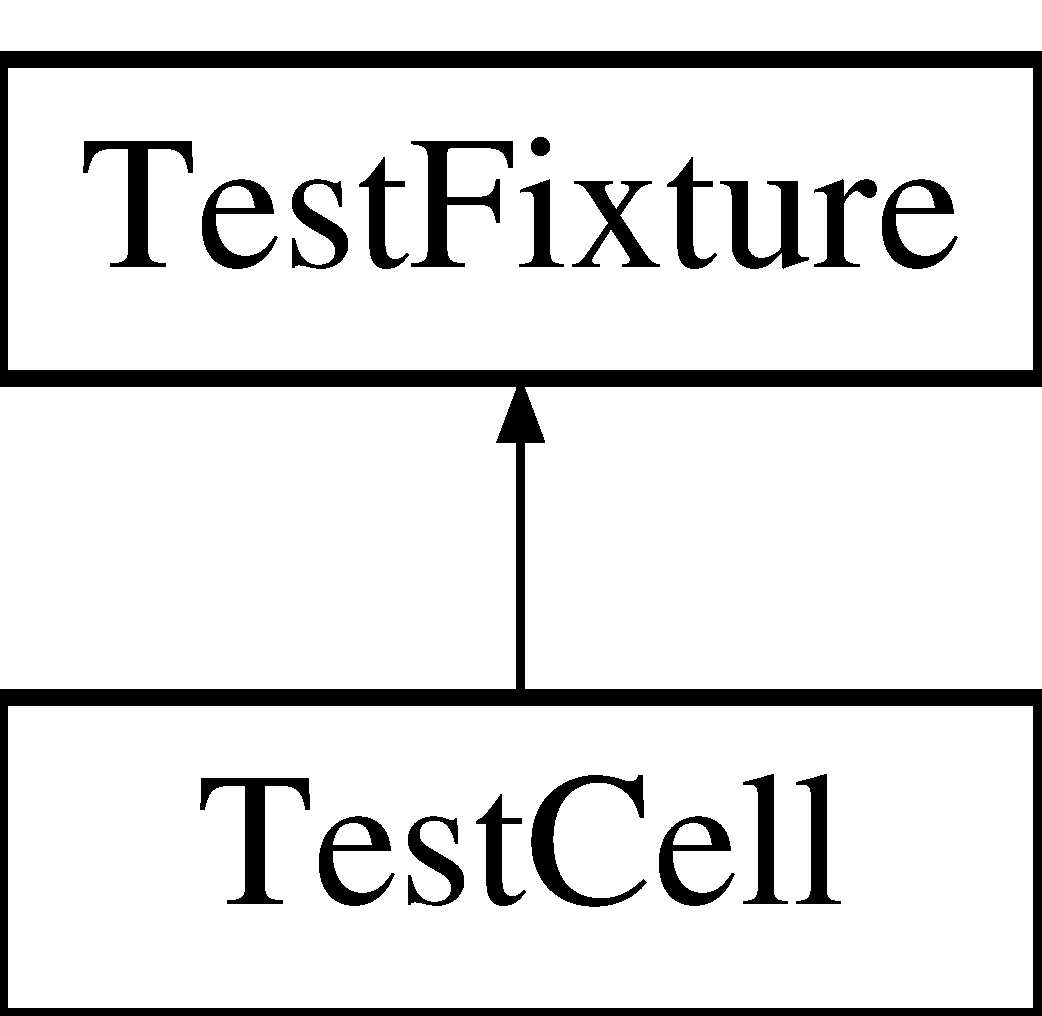
\includegraphics[height=2.000000cm]{class_test_cell}
\end{center}
\end{figure}
\subsection*{Public Member Functions}
\begin{DoxyCompactItemize}
\item 
\mbox{\Hypertarget{class_test_cell_a2b9eac7e600f08cff408df54562daa61}\label{class_test_cell_a2b9eac7e600f08cff408df54562daa61}} 
void \hyperlink{class_test_cell_a2b9eac7e600f08cff408df54562daa61}{set\+Up} ()
\begin{DoxyCompactList}\small\item\em Overide \hyperlink{class_test_cell_a2b9eac7e600f08cff408df54562daa61}{set\+Up()}, init data etc. \end{DoxyCompactList}\item 
\mbox{\Hypertarget{class_test_cell_a2ecd29c5f60aa63425c590b6399c0db0}\label{class_test_cell_a2ecd29c5f60aa63425c590b6399c0db0}} 
void \hyperlink{class_test_cell_a2ecd29c5f60aa63425c590b6399c0db0}{tear\+Down} ()
\begin{DoxyCompactList}\small\item\em Overide \hyperlink{class_test_cell_a2ecd29c5f60aa63425c590b6399c0db0}{tear\+Down()}, free allocated memory,etc. \end{DoxyCompactList}\end{DoxyCompactItemize}
\subsection*{Protected Member Functions}
\begin{DoxyCompactItemize}
\item 
void \hyperlink{class_test_cell_addf9f8fe038ba0d1543b134b04c8b3c7}{test\+Get\+Pred\+Density} ()
\begin{DoxyCompactList}\small\item\em Test method for \hyperlink{class_cell_af5ff36a4a4025053127a4ad77efb103f}{Cell\+::get\+Pred\+Density()} method. \end{DoxyCompactList}\item 
void \hyperlink{class_test_cell_ae253f8668d2328e298a94ac745086689}{test\+Get\+Prey\+Density} ()
\begin{DoxyCompactList}\small\item\em Test method for \hyperlink{class_cell_a0756af1c045a1488e2b4c2c16d87eec2}{Cell\+::get\+Prey\+Density()} method. \end{DoxyCompactList}\item 
void \hyperlink{class_test_cell_a5c2b39f6303c1ff791a000418f1edc6e}{test\+Get\+State} ()
\begin{DoxyCompactList}\small\item\em Test method for \hyperlink{class_cell_ab8c8914c6eb76fa53c4e77e692792435}{Cell\+::get\+State()} method. \end{DoxyCompactList}\item 
void \hyperlink{class_test_cell_abd30bc743823cff506c028decf6fa839}{test\+Set\+Pos\+Pred\+Density} ()
\begin{DoxyCompactList}\small\item\em Test method for \hyperlink{class_cell_adfd2fa8a4b91e18ca6195f34dbf00546}{Cell\+::set\+Pred\+Density()} method. \end{DoxyCompactList}\item 
void \hyperlink{class_test_cell_a0dd309da919dfb0e58dd371bbadffae5}{test\+Set\+Pos\+Prey\+Density} ()
\begin{DoxyCompactList}\small\item\em Test method for \hyperlink{class_cell_afd3a85027b67dfd4295e2e50253c1058}{Cell\+::set\+Prey\+Density()} method. \end{DoxyCompactList}\item 
void \hyperlink{class_test_cell_ac4beab5199462222e9b4d761d4e6c544}{test\+Set\+Neg\+Pred\+Density} ()
\begin{DoxyCompactList}\small\item\em Test method for \hyperlink{class_cell_adfd2fa8a4b91e18ca6195f34dbf00546}{Cell\+::set\+Pred\+Density()} method. \end{DoxyCompactList}\item 
void \hyperlink{class_test_cell_af9f307b147e9b64f143e21f263d35be3}{test\+Set\+Neg\+Prey\+Density} ()
\begin{DoxyCompactList}\small\item\em Test method for \hyperlink{class_cell_afd3a85027b67dfd4295e2e50253c1058}{Cell\+::set\+Prey\+Density()} method. \end{DoxyCompactList}\item 
void \hyperlink{class_test_cell_ab72285a024d96d11fabf2261400cb2b2}{test\+Set\+State\+Dry} ()
\begin{DoxyCompactList}\small\item\em Test method for \hyperlink{class_cell_ac388ff95a4d94da1497847ead859f258}{Cell\+::set\+State()} method. \end{DoxyCompactList}\item 
void \hyperlink{class_test_cell_a62ea1c29983f63087056e0fc374e9fd8}{test\+Set\+State\+Wet} ()
\begin{DoxyCompactList}\small\item\em Test method for \hyperlink{class_cell_ac388ff95a4d94da1497847ead859f258}{Cell\+::set\+State()} method. \end{DoxyCompactList}\item 
void \hyperlink{class_test_cell_afa94f24a4f02e13167bfda0dd1516272}{test\+Constructor\+Wet} ()
\begin{DoxyCompactList}\small\item\em Test method for \hyperlink{class_cell_afc0a4cece64b7689425fa81a4f6ef2e2}{Cell\+::\+Cell()} method. \end{DoxyCompactList}\item 
void \hyperlink{class_test_cell_a7c80b33b42263cfa22c782ae0bf2384c}{test\+Constructor\+Dry} ()
\begin{DoxyCompactList}\small\item\em Test method for \hyperlink{class_cell_afc0a4cece64b7689425fa81a4f6ef2e2}{Cell\+::\+Cell()} method. \end{DoxyCompactList}\item 
void \hyperlink{class_test_cell_a3c7de5784989a8b9c2f78f88aed24c52}{test\+Constructor\+Dry\+Neg\+Pred\+Density} ()
\begin{DoxyCompactList}\small\item\em Test method for \hyperlink{class_cell_afc0a4cece64b7689425fa81a4f6ef2e2}{Cell\+::\+Cell()} method. \end{DoxyCompactList}\item 
void \hyperlink{class_test_cell_adcbb2fc8a03dddd8366643f59fdb963c}{test\+Constructor\+Dry\+Neg\+Prey\+Density} ()
\begin{DoxyCompactList}\small\item\em Test method for \hyperlink{class_cell_afc0a4cece64b7689425fa81a4f6ef2e2}{Cell\+::\+Cell()} method. \end{DoxyCompactList}\item 
void \hyperlink{class_test_cell_aba7f3b946d9163abd19050db3204903e}{test\+Constructor\+Default} ()
\begin{DoxyCompactList}\small\item\em Test method for \hyperlink{class_cell_afc0a4cece64b7689425fa81a4f6ef2e2}{Cell\+::\+Cell()} method. \end{DoxyCompactList}\end{DoxyCompactItemize}


\subsection{Detailed Description}
Tests the \hyperlink{class_cell}{Cell} class. 

This test class is written using the Cpp\+Unit test framework and tests the various methods of the \hyperlink{class_cell}{Cell} class. 

\subsection{Member Function Documentation}
\mbox{\Hypertarget{class_test_cell_aba7f3b946d9163abd19050db3204903e}\label{class_test_cell_aba7f3b946d9163abd19050db3204903e}} 
\index{Test\+Cell@{Test\+Cell}!test\+Constructor\+Default@{test\+Constructor\+Default}}
\index{test\+Constructor\+Default@{test\+Constructor\+Default}!Test\+Cell@{Test\+Cell}}
\subsubsection{\texorpdfstring{test\+Constructor\+Default()}{testConstructorDefault()}}
{\footnotesize\ttfamily void Test\+Cell\+::test\+Constructor\+Default (\begin{DoxyParamCaption}{ }\end{DoxyParamCaption})\hspace{0.3cm}{\ttfamily [protected]}}



Test method for \hyperlink{class_cell_afc0a4cece64b7689425fa81a4f6ef2e2}{Cell\+::\+Cell()} method. 

Tests the default behaviour of the constructor i.\+e. if no arguments provided should create a wet cell with zero densities. \mbox{\Hypertarget{class_test_cell_a7c80b33b42263cfa22c782ae0bf2384c}\label{class_test_cell_a7c80b33b42263cfa22c782ae0bf2384c}} 
\index{Test\+Cell@{Test\+Cell}!test\+Constructor\+Dry@{test\+Constructor\+Dry}}
\index{test\+Constructor\+Dry@{test\+Constructor\+Dry}!Test\+Cell@{Test\+Cell}}
\subsubsection{\texorpdfstring{test\+Constructor\+Dry()}{testConstructorDry()}}
{\footnotesize\ttfamily void Test\+Cell\+::test\+Constructor\+Dry (\begin{DoxyParamCaption}{ }\end{DoxyParamCaption})\hspace{0.3cm}{\ttfamily [protected]}}



Test method for \hyperlink{class_cell_afc0a4cece64b7689425fa81a4f6ef2e2}{Cell\+::\+Cell()} method. 

Tests that the constructor creates a cell with correct densities if it is dry. \mbox{\Hypertarget{class_test_cell_a3c7de5784989a8b9c2f78f88aed24c52}\label{class_test_cell_a3c7de5784989a8b9c2f78f88aed24c52}} 
\index{Test\+Cell@{Test\+Cell}!test\+Constructor\+Dry\+Neg\+Pred\+Density@{test\+Constructor\+Dry\+Neg\+Pred\+Density}}
\index{test\+Constructor\+Dry\+Neg\+Pred\+Density@{test\+Constructor\+Dry\+Neg\+Pred\+Density}!Test\+Cell@{Test\+Cell}}
\subsubsection{\texorpdfstring{test\+Constructor\+Dry\+Neg\+Pred\+Density()}{testConstructorDryNegPredDensity()}}
{\footnotesize\ttfamily void Test\+Cell\+::test\+Constructor\+Dry\+Neg\+Pred\+Density (\begin{DoxyParamCaption}{ }\end{DoxyParamCaption})\hspace{0.3cm}{\ttfamily [protected]}}



Test method for \hyperlink{class_cell_afc0a4cece64b7689425fa81a4f6ef2e2}{Cell\+::\+Cell()} method. 

Tests that the constructor creates a cell with zero predator density if the predator density provided to the constructor is less than 0. \mbox{\Hypertarget{class_test_cell_adcbb2fc8a03dddd8366643f59fdb963c}\label{class_test_cell_adcbb2fc8a03dddd8366643f59fdb963c}} 
\index{Test\+Cell@{Test\+Cell}!test\+Constructor\+Dry\+Neg\+Prey\+Density@{test\+Constructor\+Dry\+Neg\+Prey\+Density}}
\index{test\+Constructor\+Dry\+Neg\+Prey\+Density@{test\+Constructor\+Dry\+Neg\+Prey\+Density}!Test\+Cell@{Test\+Cell}}
\subsubsection{\texorpdfstring{test\+Constructor\+Dry\+Neg\+Prey\+Density()}{testConstructorDryNegPreyDensity()}}
{\footnotesize\ttfamily void Test\+Cell\+::test\+Constructor\+Dry\+Neg\+Prey\+Density (\begin{DoxyParamCaption}{ }\end{DoxyParamCaption})\hspace{0.3cm}{\ttfamily [protected]}}



Test method for \hyperlink{class_cell_afc0a4cece64b7689425fa81a4f6ef2e2}{Cell\+::\+Cell()} method. 

Tests that the constructor creates a cell with zero prey density if the predator density provided to the constructor is less than 0. \mbox{\Hypertarget{class_test_cell_afa94f24a4f02e13167bfda0dd1516272}\label{class_test_cell_afa94f24a4f02e13167bfda0dd1516272}} 
\index{Test\+Cell@{Test\+Cell}!test\+Constructor\+Wet@{test\+Constructor\+Wet}}
\index{test\+Constructor\+Wet@{test\+Constructor\+Wet}!Test\+Cell@{Test\+Cell}}
\subsubsection{\texorpdfstring{test\+Constructor\+Wet()}{testConstructorWet()}}
{\footnotesize\ttfamily void Test\+Cell\+::test\+Constructor\+Wet (\begin{DoxyParamCaption}{ }\end{DoxyParamCaption})\hspace{0.3cm}{\ttfamily [protected]}}



Test method for \hyperlink{class_cell_afc0a4cece64b7689425fa81a4f6ef2e2}{Cell\+::\+Cell()} method. 

Tests that the constructor creates a cell with zero densities if it is wet. \mbox{\Hypertarget{class_test_cell_addf9f8fe038ba0d1543b134b04c8b3c7}\label{class_test_cell_addf9f8fe038ba0d1543b134b04c8b3c7}} 
\index{Test\+Cell@{Test\+Cell}!test\+Get\+Pred\+Density@{test\+Get\+Pred\+Density}}
\index{test\+Get\+Pred\+Density@{test\+Get\+Pred\+Density}!Test\+Cell@{Test\+Cell}}
\subsubsection{\texorpdfstring{test\+Get\+Pred\+Density()}{testGetPredDensity()}}
{\footnotesize\ttfamily void Test\+Cell\+::test\+Get\+Pred\+Density (\begin{DoxyParamCaption}{ }\end{DoxyParamCaption})\hspace{0.3cm}{\ttfamily [protected]}}



Test method for \hyperlink{class_cell_af5ff36a4a4025053127a4ad77efb103f}{Cell\+::get\+Pred\+Density()} method. 

Tests that the getter returns the correct predator density for the cell. \mbox{\Hypertarget{class_test_cell_ae253f8668d2328e298a94ac745086689}\label{class_test_cell_ae253f8668d2328e298a94ac745086689}} 
\index{Test\+Cell@{Test\+Cell}!test\+Get\+Prey\+Density@{test\+Get\+Prey\+Density}}
\index{test\+Get\+Prey\+Density@{test\+Get\+Prey\+Density}!Test\+Cell@{Test\+Cell}}
\subsubsection{\texorpdfstring{test\+Get\+Prey\+Density()}{testGetPreyDensity()}}
{\footnotesize\ttfamily void Test\+Cell\+::test\+Get\+Prey\+Density (\begin{DoxyParamCaption}{ }\end{DoxyParamCaption})\hspace{0.3cm}{\ttfamily [protected]}}



Test method for \hyperlink{class_cell_a0756af1c045a1488e2b4c2c16d87eec2}{Cell\+::get\+Prey\+Density()} method. 

Tests that the getter returns the correct prey density for the cell. \mbox{\Hypertarget{class_test_cell_a5c2b39f6303c1ff791a000418f1edc6e}\label{class_test_cell_a5c2b39f6303c1ff791a000418f1edc6e}} 
\index{Test\+Cell@{Test\+Cell}!test\+Get\+State@{test\+Get\+State}}
\index{test\+Get\+State@{test\+Get\+State}!Test\+Cell@{Test\+Cell}}
\subsubsection{\texorpdfstring{test\+Get\+State()}{testGetState()}}
{\footnotesize\ttfamily void Test\+Cell\+::test\+Get\+State (\begin{DoxyParamCaption}{ }\end{DoxyParamCaption})\hspace{0.3cm}{\ttfamily [protected]}}



Test method for \hyperlink{class_cell_ab8c8914c6eb76fa53c4e77e692792435}{Cell\+::get\+State()} method. 

Tests that the getter returns the state for the cell. \mbox{\Hypertarget{class_test_cell_ac4beab5199462222e9b4d761d4e6c544}\label{class_test_cell_ac4beab5199462222e9b4d761d4e6c544}} 
\index{Test\+Cell@{Test\+Cell}!test\+Set\+Neg\+Pred\+Density@{test\+Set\+Neg\+Pred\+Density}}
\index{test\+Set\+Neg\+Pred\+Density@{test\+Set\+Neg\+Pred\+Density}!Test\+Cell@{Test\+Cell}}
\subsubsection{\texorpdfstring{test\+Set\+Neg\+Pred\+Density()}{testSetNegPredDensity()}}
{\footnotesize\ttfamily void Test\+Cell\+::test\+Set\+Neg\+Pred\+Density (\begin{DoxyParamCaption}{ }\end{DoxyParamCaption})\hspace{0.3cm}{\ttfamily [protected]}}



Test method for \hyperlink{class_cell_adfd2fa8a4b91e18ca6195f34dbf00546}{Cell\+::set\+Pred\+Density()} method. 

Tests that the setter sets the correct density for negative arguments. \mbox{\Hypertarget{class_test_cell_af9f307b147e9b64f143e21f263d35be3}\label{class_test_cell_af9f307b147e9b64f143e21f263d35be3}} 
\index{Test\+Cell@{Test\+Cell}!test\+Set\+Neg\+Prey\+Density@{test\+Set\+Neg\+Prey\+Density}}
\index{test\+Set\+Neg\+Prey\+Density@{test\+Set\+Neg\+Prey\+Density}!Test\+Cell@{Test\+Cell}}
\subsubsection{\texorpdfstring{test\+Set\+Neg\+Prey\+Density()}{testSetNegPreyDensity()}}
{\footnotesize\ttfamily void Test\+Cell\+::test\+Set\+Neg\+Prey\+Density (\begin{DoxyParamCaption}{ }\end{DoxyParamCaption})\hspace{0.3cm}{\ttfamily [protected]}}



Test method for \hyperlink{class_cell_afd3a85027b67dfd4295e2e50253c1058}{Cell\+::set\+Prey\+Density()} method. 

Tests that the setter sets the correct density for negative arguments. \mbox{\Hypertarget{class_test_cell_abd30bc743823cff506c028decf6fa839}\label{class_test_cell_abd30bc743823cff506c028decf6fa839}} 
\index{Test\+Cell@{Test\+Cell}!test\+Set\+Pos\+Pred\+Density@{test\+Set\+Pos\+Pred\+Density}}
\index{test\+Set\+Pos\+Pred\+Density@{test\+Set\+Pos\+Pred\+Density}!Test\+Cell@{Test\+Cell}}
\subsubsection{\texorpdfstring{test\+Set\+Pos\+Pred\+Density()}{testSetPosPredDensity()}}
{\footnotesize\ttfamily void Test\+Cell\+::test\+Set\+Pos\+Pred\+Density (\begin{DoxyParamCaption}{ }\end{DoxyParamCaption})\hspace{0.3cm}{\ttfamily [protected]}}



Test method for \hyperlink{class_cell_adfd2fa8a4b91e18ca6195f34dbf00546}{Cell\+::set\+Pred\+Density()} method. 

Tests that the setter sets the correct density for positive arguments. \mbox{\Hypertarget{class_test_cell_a0dd309da919dfb0e58dd371bbadffae5}\label{class_test_cell_a0dd309da919dfb0e58dd371bbadffae5}} 
\index{Test\+Cell@{Test\+Cell}!test\+Set\+Pos\+Prey\+Density@{test\+Set\+Pos\+Prey\+Density}}
\index{test\+Set\+Pos\+Prey\+Density@{test\+Set\+Pos\+Prey\+Density}!Test\+Cell@{Test\+Cell}}
\subsubsection{\texorpdfstring{test\+Set\+Pos\+Prey\+Density()}{testSetPosPreyDensity()}}
{\footnotesize\ttfamily void Test\+Cell\+::test\+Set\+Pos\+Prey\+Density (\begin{DoxyParamCaption}{ }\end{DoxyParamCaption})\hspace{0.3cm}{\ttfamily [protected]}}



Test method for \hyperlink{class_cell_afd3a85027b67dfd4295e2e50253c1058}{Cell\+::set\+Prey\+Density()} method. 

Tests that the setter sets the correct density for positive arguments. \mbox{\Hypertarget{class_test_cell_ab72285a024d96d11fabf2261400cb2b2}\label{class_test_cell_ab72285a024d96d11fabf2261400cb2b2}} 
\index{Test\+Cell@{Test\+Cell}!test\+Set\+State\+Dry@{test\+Set\+State\+Dry}}
\index{test\+Set\+State\+Dry@{test\+Set\+State\+Dry}!Test\+Cell@{Test\+Cell}}
\subsubsection{\texorpdfstring{test\+Set\+State\+Dry()}{testSetStateDry()}}
{\footnotesize\ttfamily void Test\+Cell\+::test\+Set\+State\+Dry (\begin{DoxyParamCaption}{ }\end{DoxyParamCaption})\hspace{0.3cm}{\ttfamily [protected]}}



Test method for \hyperlink{class_cell_ac388ff95a4d94da1497847ead859f258}{Cell\+::set\+State()} method. 

Tests that the setter sets the correct state for Cell\+::\+Dry arguments. \mbox{\Hypertarget{class_test_cell_a62ea1c29983f63087056e0fc374e9fd8}\label{class_test_cell_a62ea1c29983f63087056e0fc374e9fd8}} 
\index{Test\+Cell@{Test\+Cell}!test\+Set\+State\+Wet@{test\+Set\+State\+Wet}}
\index{test\+Set\+State\+Wet@{test\+Set\+State\+Wet}!Test\+Cell@{Test\+Cell}}
\subsubsection{\texorpdfstring{test\+Set\+State\+Wet()}{testSetStateWet()}}
{\footnotesize\ttfamily void Test\+Cell\+::test\+Set\+State\+Wet (\begin{DoxyParamCaption}{ }\end{DoxyParamCaption})\hspace{0.3cm}{\ttfamily [protected]}}



Test method for \hyperlink{class_cell_ac388ff95a4d94da1497847ead859f258}{Cell\+::set\+State()} method. 

Tests that the setter sets the state for Cell\+::\+Wet arguments. 

The documentation for this class was generated from the following files\+:\begin{DoxyCompactItemize}
\item 
test/Test\+Cell.\+hpp\item 
test/Test\+Cell.\+cpp\end{DoxyCompactItemize}

\hypertarget{class_test_grid}{}\section{Test\+Grid Class Reference}
\label{class_test_grid}\index{Test\+Grid@{Test\+Grid}}
Inheritance diagram for Test\+Grid\+:\begin{figure}[H]
\begin{center}
\leavevmode
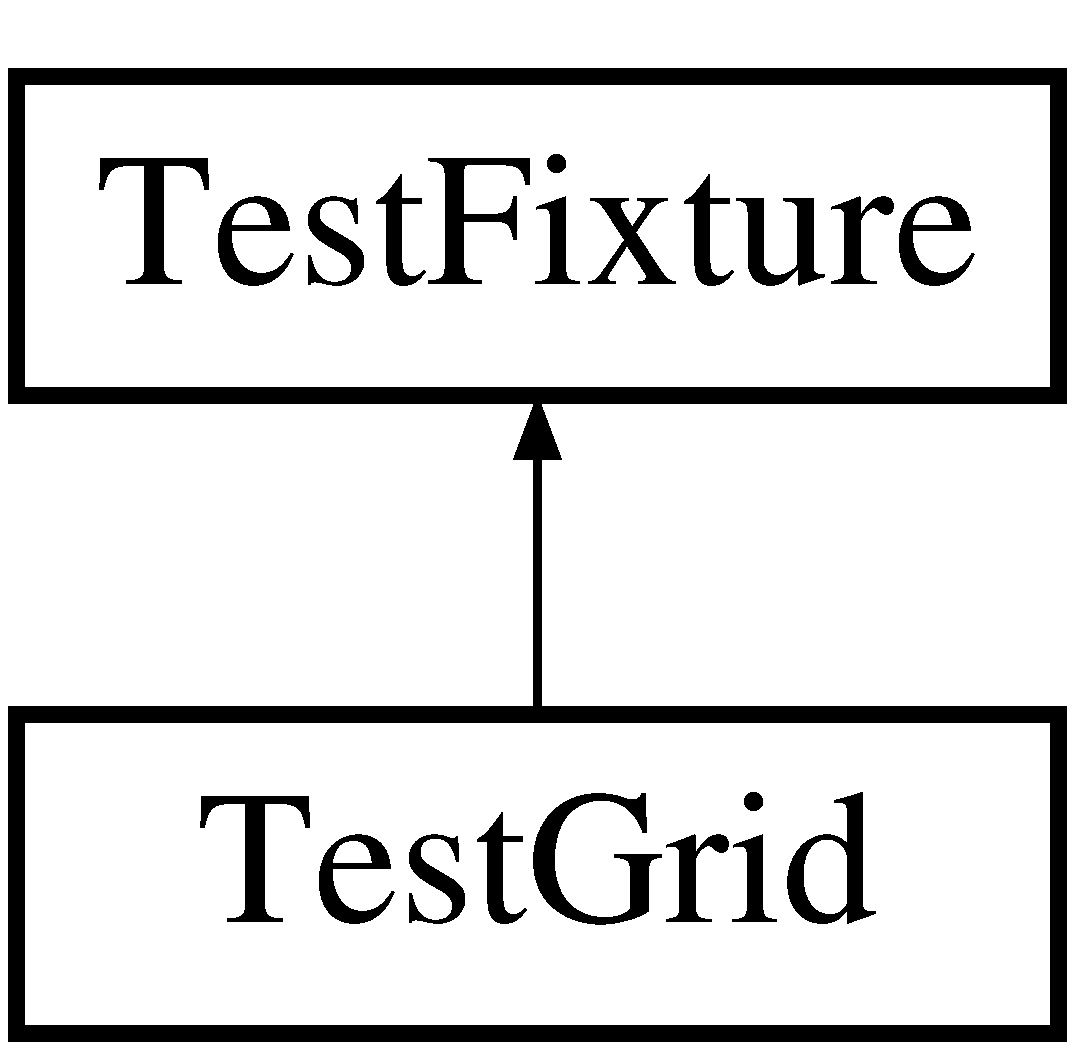
\includegraphics[height=2.000000cm]{class_test_grid}
\end{center}
\end{figure}
\subsection*{Public Member Functions}
\begin{DoxyCompactItemize}
\item 
\mbox{\Hypertarget{class_test_grid_afd080168a37a3a3374fa11b0a48ef1bf}\label{class_test_grid_afd080168a37a3a3374fa11b0a48ef1bf}} 
void {\bfseries set\+Up} ()
\item 
\mbox{\Hypertarget{class_test_grid_adf786b04244594688bf871ded5cbf860}\label{class_test_grid_adf786b04244594688bf871ded5cbf860}} 
void {\bfseries tear\+Down} ()
\item 
\mbox{\Hypertarget{class_test_grid_a5f4d88062bad9698b14e99067cb6a3bf}\label{class_test_grid_a5f4d88062bad9698b14e99067cb6a3bf}} 
void {\bfseries test\+Constructor1} ()
\item 
\mbox{\Hypertarget{class_test_grid_accd340be5dc916a1769bab50471c1cc8}\label{class_test_grid_accd340be5dc916a1769bab50471c1cc8}} 
void {\bfseries test\+Constructor2} ()
\end{DoxyCompactItemize}


The documentation for this class was generated from the following files\+:\begin{DoxyCompactItemize}
\item 
test/Test\+Grid.\+hpp\item 
test/Test\+Grid.\+cpp\end{DoxyCompactItemize}

\hypertarget{class_test_update_grid}{}\section{Test\+Update\+Grid Class Reference}
\label{class_test_update_grid}\index{Test\+Update\+Grid@{Test\+Update\+Grid}}


Tests the update\+Grid function.  




{\ttfamily \#include $<$Test\+Update\+Grid.\+hpp$>$}

Inheritance diagram for Test\+Update\+Grid\+:\begin{figure}[H]
\begin{center}
\leavevmode
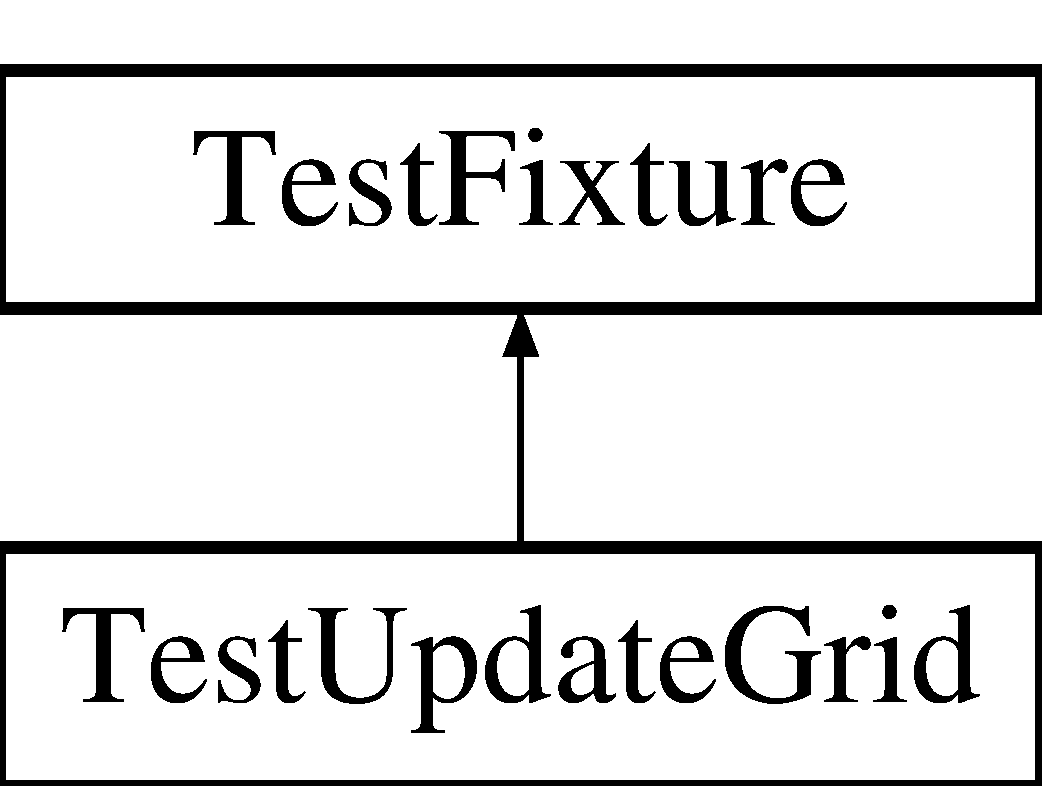
\includegraphics[height=2.000000cm]{class_test_update_grid}
\end{center}
\end{figure}
\subsection*{Public Member Functions}
\begin{DoxyCompactItemize}
\item 
\mbox{\Hypertarget{class_test_update_grid_a0a50fd0d318cb2fe27dfc7fa5c8a0f33}\label{class_test_update_grid_a0a50fd0d318cb2fe27dfc7fa5c8a0f33}} 
void \hyperlink{class_test_update_grid_a0a50fd0d318cb2fe27dfc7fa5c8a0f33}{set\+Up} ()
\begin{DoxyCompactList}\small\item\em Override \hyperlink{class_test_update_grid_a0a50fd0d318cb2fe27dfc7fa5c8a0f33}{set\+Up()}, initialise test cases etc. \end{DoxyCompactList}\item 
\mbox{\Hypertarget{class_test_update_grid_a482b2a4a0f2fd8252032bde4b28c3778}\label{class_test_update_grid_a482b2a4a0f2fd8252032bde4b28c3778}} 
void \hyperlink{class_test_update_grid_a482b2a4a0f2fd8252032bde4b28c3778}{tear\+Down} ()
\begin{DoxyCompactList}\small\item\em Override \hyperlink{class_test_update_grid_a482b2a4a0f2fd8252032bde4b28c3778}{tear\+Down()}, free allocated memory in test cases, etc. \end{DoxyCompactList}\end{DoxyCompactItemize}
\subsection*{Protected Member Functions}
\begin{DoxyCompactItemize}
\item 
void \hyperlink{class_test_update_grid_a96aa33a3e1362f9a24237c234a13f3b9}{test\+Wet\+Grid\+Updated} ()
\begin{DoxyCompactList}\small\item\em Test method for update\+Grid() function. \end{DoxyCompactList}\item 
void \hyperlink{class_test_update_grid_ac9edeb07286572669ab1464895f3f452}{test\+Zero\+Density\+Grid\+Updated} ()
\begin{DoxyCompactList}\small\item\em Test method for update\+Grid() function. \end{DoxyCompactList}\item 
void \hyperlink{class_test_update_grid_a5ae8a15bf6d4fc2429b9e0b0946b08c8}{test\+Realistic\+Grid\+Updated} ()
\begin{DoxyCompactList}\small\item\em Test method for update\+Grid() function. \end{DoxyCompactList}\end{DoxyCompactItemize}


\subsection{Detailed Description}
Tests the update\+Grid function. 

This test class is written using the Cpp\+Unit test framework and tests the function that updates the grid. 

\subsection{Member Function Documentation}
\mbox{\Hypertarget{class_test_update_grid_a5ae8a15bf6d4fc2429b9e0b0946b08c8}\label{class_test_update_grid_a5ae8a15bf6d4fc2429b9e0b0946b08c8}} 
\index{Test\+Update\+Grid@{Test\+Update\+Grid}!test\+Realistic\+Grid\+Updated@{test\+Realistic\+Grid\+Updated}}
\index{test\+Realistic\+Grid\+Updated@{test\+Realistic\+Grid\+Updated}!Test\+Update\+Grid@{Test\+Update\+Grid}}
\subsubsection{\texorpdfstring{test\+Realistic\+Grid\+Updated()}{testRealisticGridUpdated()}}
{\footnotesize\ttfamily void Test\+Update\+Grid\+::test\+Realistic\+Grid\+Updated (\begin{DoxyParamCaption}{ }\end{DoxyParamCaption})\hspace{0.3cm}{\ttfamily [protected]}}



Test method for update\+Grid() function. 

Tests that the function correctly updates a grid that initially has non-\/zero densities. \mbox{\Hypertarget{class_test_update_grid_a96aa33a3e1362f9a24237c234a13f3b9}\label{class_test_update_grid_a96aa33a3e1362f9a24237c234a13f3b9}} 
\index{Test\+Update\+Grid@{Test\+Update\+Grid}!test\+Wet\+Grid\+Updated@{test\+Wet\+Grid\+Updated}}
\index{test\+Wet\+Grid\+Updated@{test\+Wet\+Grid\+Updated}!Test\+Update\+Grid@{Test\+Update\+Grid}}
\subsubsection{\texorpdfstring{test\+Wet\+Grid\+Updated()}{testWetGridUpdated()}}
{\footnotesize\ttfamily void Test\+Update\+Grid\+::test\+Wet\+Grid\+Updated (\begin{DoxyParamCaption}{ }\end{DoxyParamCaption})\hspace{0.3cm}{\ttfamily [protected]}}



Test method for update\+Grid() function. 

Tests that the function correctly updates a grid that is wet everywhere. \mbox{\Hypertarget{class_test_update_grid_ac9edeb07286572669ab1464895f3f452}\label{class_test_update_grid_ac9edeb07286572669ab1464895f3f452}} 
\index{Test\+Update\+Grid@{Test\+Update\+Grid}!test\+Zero\+Density\+Grid\+Updated@{test\+Zero\+Density\+Grid\+Updated}}
\index{test\+Zero\+Density\+Grid\+Updated@{test\+Zero\+Density\+Grid\+Updated}!Test\+Update\+Grid@{Test\+Update\+Grid}}
\subsubsection{\texorpdfstring{test\+Zero\+Density\+Grid\+Updated()}{testZeroDensityGridUpdated()}}
{\footnotesize\ttfamily void Test\+Update\+Grid\+::test\+Zero\+Density\+Grid\+Updated (\begin{DoxyParamCaption}{ }\end{DoxyParamCaption})\hspace{0.3cm}{\ttfamily [protected]}}



Test method for update\+Grid() function. 

Tests that the function correctly updates a grid that initially has zero densities everywhere. 

The documentation for this class was generated from the following files\+:\begin{DoxyCompactItemize}
\item 
test/\hyperlink{_test_update_grid_8hpp}{Test\+Update\+Grid.\+hpp}\item 
test/Test\+Update\+Grid.\+cpp\end{DoxyCompactItemize}

\chapter{File Documentation}
\hypertarget{_cell_8hpp}{}\section{src/\+Cell.hpp File Reference}
\label{_cell_8hpp}\index{src/\+Cell.\+hpp@{src/\+Cell.\+hpp}}
\subsection*{Classes}
\begin{DoxyCompactItemize}
\item 
class \hyperlink{class_cell}{Cell}
\begin{DoxyCompactList}\small\item\em Models a single cell. \end{DoxyCompactList}\end{DoxyCompactItemize}

\hypertarget{_grid_8hpp}{}\section{src/\+Grid.hpp File Reference}
\label{_grid_8hpp}\index{src/\+Grid.\+hpp@{src/\+Grid.\+hpp}}
{\ttfamily \#include \char`\"{}Cell.\+hpp\char`\"{}}\newline
{\ttfamily \#include $<$fstream$>$}\newline
{\ttfamily \#include $<$cassert$>$}\newline
{\ttfamily \#include $<$iostream$>$}\newline
{\ttfamily \#include $<$random$>$}\newline
{\ttfamily \#include $<$stdexcept$>$}\newline
\subsection*{Classes}
\begin{DoxyCompactItemize}
\item 
class \hyperlink{class_grid}{Grid}
\begin{DoxyCompactList}\small\item\em Models a 2D landscape of cells. \end{DoxyCompactList}\end{DoxyCompactItemize}

\hypertarget{update_grid_8hpp}{}\section{src/update\+Grid.hpp File Reference}
\label{update_grid_8hpp}\index{src/update\+Grid.\+hpp@{src/update\+Grid.\+hpp}}


Updates the grid by one timestep.  


{\ttfamily \#include \char`\"{}Grid.\+hpp\char`\"{}}\newline
\subsection*{Functions}
\begin{DoxyCompactItemize}
\item 
\mbox{\Hypertarget{update_grid_8hpp_a0e191f0c2c19b666638c4c6936edc10f}\label{update_grid_8hpp_a0e191f0c2c19b666638c4c6936edc10f}} 
\hyperlink{class_grid}{Grid} {\bfseries update\+Grid} (\hyperlink{class_grid}{Grid} \&grid, double r, double a, double b, double m, double k, double l, double deltaT)
\end{DoxyCompactItemize}


\subsection{Detailed Description}
Updates the grid by one timestep. 

Function to update the densities of predator and prey in a grid instance according to the differential equation specified in the coursework pdf.


\begin{DoxyParams}{Parameters}
{\em grid} & \hyperlink{class_grid}{Grid} reference instance to be updated.\\
\hline
{\em r} & double instance representing the birth rate of hares (prey).\\
\hline
{\em a} & double instance representing the predation rate at which pumas (predators).\\
\hline
{\em b} & double instance representing the birth rate of pumas (predators) per one hare (prey) eaten.\\
\hline
{\em m} & double instance representing the puma (predator) mortality rate.\\
\hline
{\em k} & double instance representing the diffusion rate for hares (prey).\\
\hline
{\em l} & double instance representing the diffusion rate for pumas (predators).\\
\hline
{\em deltaT} & double instance representing the timestep value.\\
\hline
\end{DoxyParams}
\begin{DoxyReturn}{Returns}
\hyperlink{class_grid}{Grid} instance which is the original grid updated by one timestep. 
\end{DoxyReturn}

%--- End generated contents ---

% Index
\backmatter
\newpage
\phantomsection
\clearemptydoublepage
\addcontentsline{toc}{chapter}{Index}
\printindex

\end{document}
